\documentclass[12pt,a4paper]{article}

\renewcommand*\contentsname{Sadržaj}
\renewcommand{\figurename}{Slika}
\renewcommand{\tablename}{Tabela}
\renewcommand\refname{Reference}
\renewcommand{\arraystretch}{1.5}

\usepackage[margin=0.85in]{geometry}
\usepackage{graphicx}
\usepackage{float}
\usepackage{listings}
\usepackage{multirow}
\usepackage{xcolor}
\usepackage{colortbl}
\usepackage{color}

\lstloadlanguages{C,C++,csh,Java}

\definecolor{red}{rgb}{0.6,0,0} 
\definecolor{blue}{rgb}{0,0,0.6}
\definecolor{green}{rgb}{0,0.8,0}
\definecolor{cyan}{rgb}{0.0,0.6,0.6}
\definecolor{cloudwhite}{rgb}{0.9412, 0.9608, 0.8471}

\lstset{
language=csh,
basicstyle=\footnotesize\ttfamily,
numbers=left,
numberstyle=\tiny,
numbersep=5pt,
tabsize=2,
extendedchars=true,
breaklines=true,
frame=b,
stringstyle=\color{blue}\ttfamily,
showspaces=false,
showtabs=false,
xleftmargin=17pt,
framexleftmargin=17pt,
framexrightmargin=5pt,
framexbottommargin=4pt,
commentstyle=\color{green},
morecomment=[l]{//}, %use comment-line-style!
morecomment=[s]{/*}{*/}, %for multiline comments
showstringspaces=false,
morekeywords={ abstract, event, new, struct,
as, explicit, null, switch,
base, extern, object, this,
bool, false, operator, throw,
break, finally, out, true,
byte, fixed, override, try,
case, float, params, typeof,
catch, for, private, uint,
char, foreach, protected, ulong,
checked, goto, public, unchecked,
class, if, readonly, unsafe,
const, implicit, ref, ushort,
continue, in, return, using,
decimal, int, sbyte, virtual,
default, interface, sealed, volatile,
delegate, internal, short, void,
do, is, sizeof, while,
double, lock, stackalloc,
else, long, static,
enum, namespace, string},
keywordstyle=\color{cyan},
identifierstyle=\color{red},
backgroundcolor=\color{cloudwhite},
}

\usepackage{caption}
\DeclareCaptionFont{white}{\color{white}}
\DeclareCaptionFormat{listing}{\colorbox{blue}{\parbox{\textwidth}{\hspace{15pt}#1#2#3}}}
\captionsetup[lstlisting]{format=listing,labelfont=white,textfont=white, singlelinecheck=false, margin=0pt, font={bf,footnotesize}}

\newcolumntype{a}{>{\columncolor{green}}c}
\newcolumntype{b}{>{\columncolor{lime}}c}
\newcolumntype{d}{>{\columncolor{teal}}c}
\newcolumntype{e}{>{\columncolor{cyan}}c}
\newcolumntype{f}{>{\columncolor{violet}}c}
\newcolumntype{P}[1]{>{\centering\arraybackslash}p{#1}}

\begin{document}

\begin{titlepage}
	\centering
	{\scshape Univerzitet u Sarajevu \par}
	{\scshape Elektrotehnički Fakultet \par}
	{\scshape Odsjek za Računarstvo i Informatiku \par}
	\vspace{2cm}
	{\Large\scshape Seminarski rad iz predmeta Multimedijalni Sistemi\par}
	\vspace{2.5cm}
	{\huge\bfseries Konverzija RGB Slika u Zvučni Sadržaj\par}
	\vspace{2.5cm}
	\Large Studenti: \par
	{\Large\itshape \textsc{Muftić} Belma, 1423/17260\par}
	{\Large\itshape \textsc{Kulović} Nejra, 1519/17484\par}
	{\Large\itshape \textsc{Krupalija} Ehlimana, 1431/17461\par}
	\vfill
	Predmetni nastavnik:\par
	r. prof. dr. \textsc{Haris Šupić}, dipl. ing. el.
	\vfill
	{\large Februar, 2019\par}
\end{titlepage}

\pagenumbering{gobble}

\section*{Definicija Zadatka}

U ovom radu opisan je postupak pretvaranja slika u boji u zvučni sadržaj. U ovu svrhu prvo je neophodno izdvojiti boje iz slike (budući da se rezultujuće zvučne datoteke razlikuju na osnovu različitog udjela boja u slici), zatim je potrebno na adekvatan način dodijeliti određeni ton (od mogućih 128) nijansama boja, te kreirati zvučnu datoteku u \textit{.mid} formatu. Kako bi se ovaj postupak demonstrirao, napravljena je \textit{Windows Forms} aplikacija koristeći programski jezik \texttt{C\#}, koja korisnicima omogućava odabir slike u boji za konverziju, pokretanje postupka konverzije te puštanje rezultujućeg zvučnog sadržaja. \\

U radu su detaljno opisane sve faze konverzije, uključujući razlaganje slike na \textit{color channels}, mapiranje različitih boja u karakteristične frekvencije zvuka (tonove), odabir audio formata koji je najpogodniji za ovakvu konverziju te sam postupak kreiranja audio \textit{file}-ova u odabranom formatu. Opisan je način implementacije aplikacije koja vrši konverziju, odnosno način na koji se slika razlaže na \textit{color channels}, boje dodjeljuju frekvencijama, te date frekvencije koriste kako bi se kreirao audio \textit{file} koji korisnici zatim mogu slušati. \\

Na kraju je opisan značaj ovakvog postupka, odnosno njegova moguća primjena u praksi za omogućavanje diferenciranja (i općenito identifikacije) različitih boja za ljude koji nisu u stanju da vide boje (ahromatopsija) ili razlikuju pojedine boje (daltonizam), te preciznost same konverzije.

\newpage

\section*{Izjava o Doprinosu Članova Tima Pri Izradi Seminarskog Rada}

\begin{table}[H]
\centering
\begin{tabular}{| c | p{12 cm} |}
\hline
\textbf{Član tima}					& \textbf{Aktivnosti}		\\ \hline
\multirow{4}{*}{Belma Muftić}		& \textit{Analiza problema}: Definicija teme \\
								& \textit{Osmišljavanje rješenja}: Pronalazak rješenja za problem pretvaranja \textit{color channels} u oblik pogodan za pretvaranje u zvučni sadržaj \\
								& \textit{Praktična implementacija}: Dio rastavljanja slike na \textit{color channels} i pretvaranje u ekvivalentne frekvencije zvuka \\
								& \textit{Pisanje teksta}: Za prethodno navedeni dio problema \\ \hline
\multirow{4}{*}{Nejra Kulović}		& \textit{Analiza problema}: Odabir tehnologije za razvoj rješenja \\
								& \textit{Osmišljavanje rješenja}: Ideja za rješavanje problema dodjeljivanja odgovarajućih frekvencija zvuka dekodiranim bojama \\
								& \textit{Praktična implementacija}: Aplikacija koja objedinjuje zasebne dijelove za manipulisanje slikom i zvukom te njihovo spajanje i usklađivanje \\
								& \textit{Pisanje teksta}: Za prethodno navedeni dio problema \\ \hline
\multirow{4}{*}{Ehlimana Krupalija} & \textit{Analiza problema}: Odabir vrste protokola za rezultujuće zvučne \textit{file}-ove \\
								& \textit{Osmišljavanje rješenja}: Prilagođavanje \textit{.mid} formata primjeni te pretvaranje dodijeljenih frekvencija u audio format \\
								& \textit{Praktična implementacija}: Dio definisanja dijelova MIDI \textit{file}-a, ubacivanja zvučnog sadržaja i kreiranja \textit{.mid file}-a \\
								& \textit{Pisanje teksta}: Za prethodno navedeni dio problema \\ \hline
\end{tabular}
\caption{Opis aktivnosti članova tima pri rješavanju problema}
\end{table}

\newpage

\tableofcontents

\newpage

\pagenumbering{arabic}
\setcounter{page}{1}

\section{Uvod}

\subsection{Postavka problema}

Problem koji će biti riješen u okviru ovog rada je pronalazak načina da se premosti prepreka koju predstavlja nemogućnost viđenja ili razlikovanja boja. Budući da osobe koji nisu u stanju razlikovati ili vidjeti boje vide slike u boji kao da su \textit{grayscale}, neophodno je izvršiti ekstrakciju onih elemenata koje oni ne vide - boje - te njihovu konverziju u sadržaj koji će moći razlikovati, što je u najvećem broju slučajeva zvuk. Iz tog razloga izvršiti će se postupak konverzije slika u boji u zvučni sadržaj. \\

U ovu svrhu potrebno je definisati tri glavne faze konverzije:

\begin{enumerate}

\item \underline{Izdvajanje boja iz slike}, odnosno adekvatno razlaganje slike na određeni broj nijansi;
\item \underline{Mapiranje pojedinih boja u frekvencije zvuka};
\item \underline{Kreiranje audio \textit{file}-a} na osnovu informacija o tonovima od kojih se ista treba sastojati.

\end{enumerate}

U nastavku će biti detaljno objašnjene sve faze konverzije, odnosno način ekstrakcije boja iz slike, njihovog mapiranja u različite frekvencije zvuka (koje će predstavljati način razlikovanja boja) te spajanja različitih boja u jedinstven audio \textit{file} koji će zatim biti moguće reproducirati te na taj način putem slušnog organa omogućiti identifikaciju različitih boja.

\subsection{Modeli boja}

Model boja je način da se predstavi boja, bilo na ekranima ili prilikom printanja \cite{bels1}, tako što se kombinuje skup primarnih boja. Postoje razni modeli, no neki od najznačajnijih su \cite{bels2}:

\begin{itemize}

\item RGB (\textit{Red, Green, Blue});
\item CMYK (\textit{Cyan, Magenta, Yellow, Black});
\item \textit{Grayscale};
\item HSV (\textit{Hue, Saturation, Value}).

\end{itemize}

\subsubsection{RGB model boja}

Ovaj model se koristi prilikom prikaza slike na ekranima, te se još naziva i \textbf{aditivnim modelom} jer koristi svjetlost da se prikaže boja \cite{bels2}. Slika se sastoji od tri kanala boja (\textit{color channels}) čije vrijednosti se kreću od 0 do 255 uključivo: crvena, zelena i plava. Kada svi kanali imaju vrijednost 0, tada se kreira crna boja, a kada su vrijednosti 255, tada se kreira bijela boja. ''Čista'' plava/crvena/zelena boja nastaje kada se vrijednosti ostale dvije boje postave na 0, vrijednost čiste boje na 255, dok se ostali spektar boja dobija kombinacijom ove tri boje \cite{bels1}. Kao rezultat, moguće je predstaviti \textbf{16.7 miliona različitih boja} \cite{bels2} ovim modelom. \\

Prikaz RGB slike na digitalnim ekranima se vrši uz pomoć \textbf{tri odgovarajuće obojene svjetlosne zrake} koje je potrebno ''preklopiti'' (\textit{superimpose}) jednu preko druge. Kada nijedna zraka nema intenzitet, onda se kreira crna boja, dok puni intenzitet sve tri boje kreira bijelu boju (analogno numeričkim vrijednostima) \cite{bels2}. Na Slici \ref{rgb} prikazan je dijagram RGB modela.

\begin{figure}[H]

\center
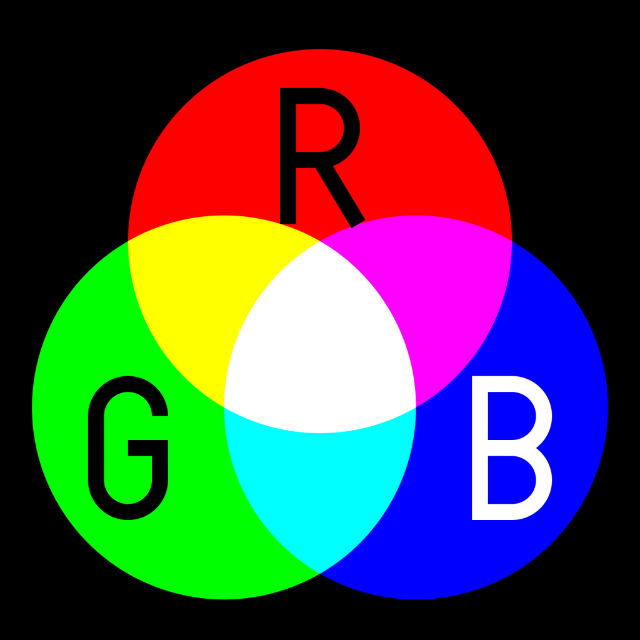
\includegraphics[scale=0.75]{../res/rgb.png}
\caption{RGB model boja \cite{bels3}}
\label{rgb}

\end{figure}

\subsubsection{CMYK model boja}

Za razliku od RGB modela, ovaj model je \textbf{subtraktivni model}, kako koristi grafičke boje za prikaz, što ga čini pogodnim za printanje. Kanali koji čine ovaj model jesu cijan, purpurno crvena, žuta, te crna, i koriste se tako što se na bijelu pozadinu ''maskiraju'' boje, te se tako smanjuje svjetlost koja se reflektuje, zbog čega se i naziva subtraktivnim modelom. Crna se uvodi jer mješavina ostale tri boje ne daje čistu crnu boju \cite{bels2}, a na Slici \ref	{cmyk} prikazan je dijagram ovog modela.

\begin{figure}[H]

\center

\includegraphics[scale=0.75]{../res/cmyk.PNG}
\caption{CMYK model boja \cite{bels4}}
\label{cmyk}

\end{figure}

\subsubsection{\textit{Grayscale} model boja}

\textit{Grayscale} slika jeste slika koja sadrži samo nijanse sive boje, dakle ovaj model ima \textbf{samo jedan kanal} koji nosi informaciju o intenzitetu piksela. Slično kao kod RGB modela, vrijednost 0 predstavlja crnu boju, dok vrijednost 255 daje bijelu boju \cite{bels2}.

\subsubsection{HSV model boja}

HSV predstavlja trodimenzionalni model boja koji opisuje odnose između boja, te koji se sastoji od tri kanala: \textbf{nijansa}, \textbf{zasićenost} i \textbf{vrijednost}. Na Slici \ref{hsv} nalazi se 3D prikaz ovog modela, gdje je očito da centar točka predstavlja bijelu boju, krajevi predstavljaju crnu boju, dok se ostale boje nalaze između. Ugao od ose predstavlja nijansu (što znači da vrijednosti idu od 0 do 360), udaljenost od ose predstavlja zasićenost boje, dok je nijasnsa predstavljena udaljenošću duž ose. Vrijedi napomenuti da pored HSV modela postoji i \textbf{HSL model}, gdje se umjesto nijanse nalazi količina svjetlosti boje \cite{bels2}.

\begin{figure}[H]

\center
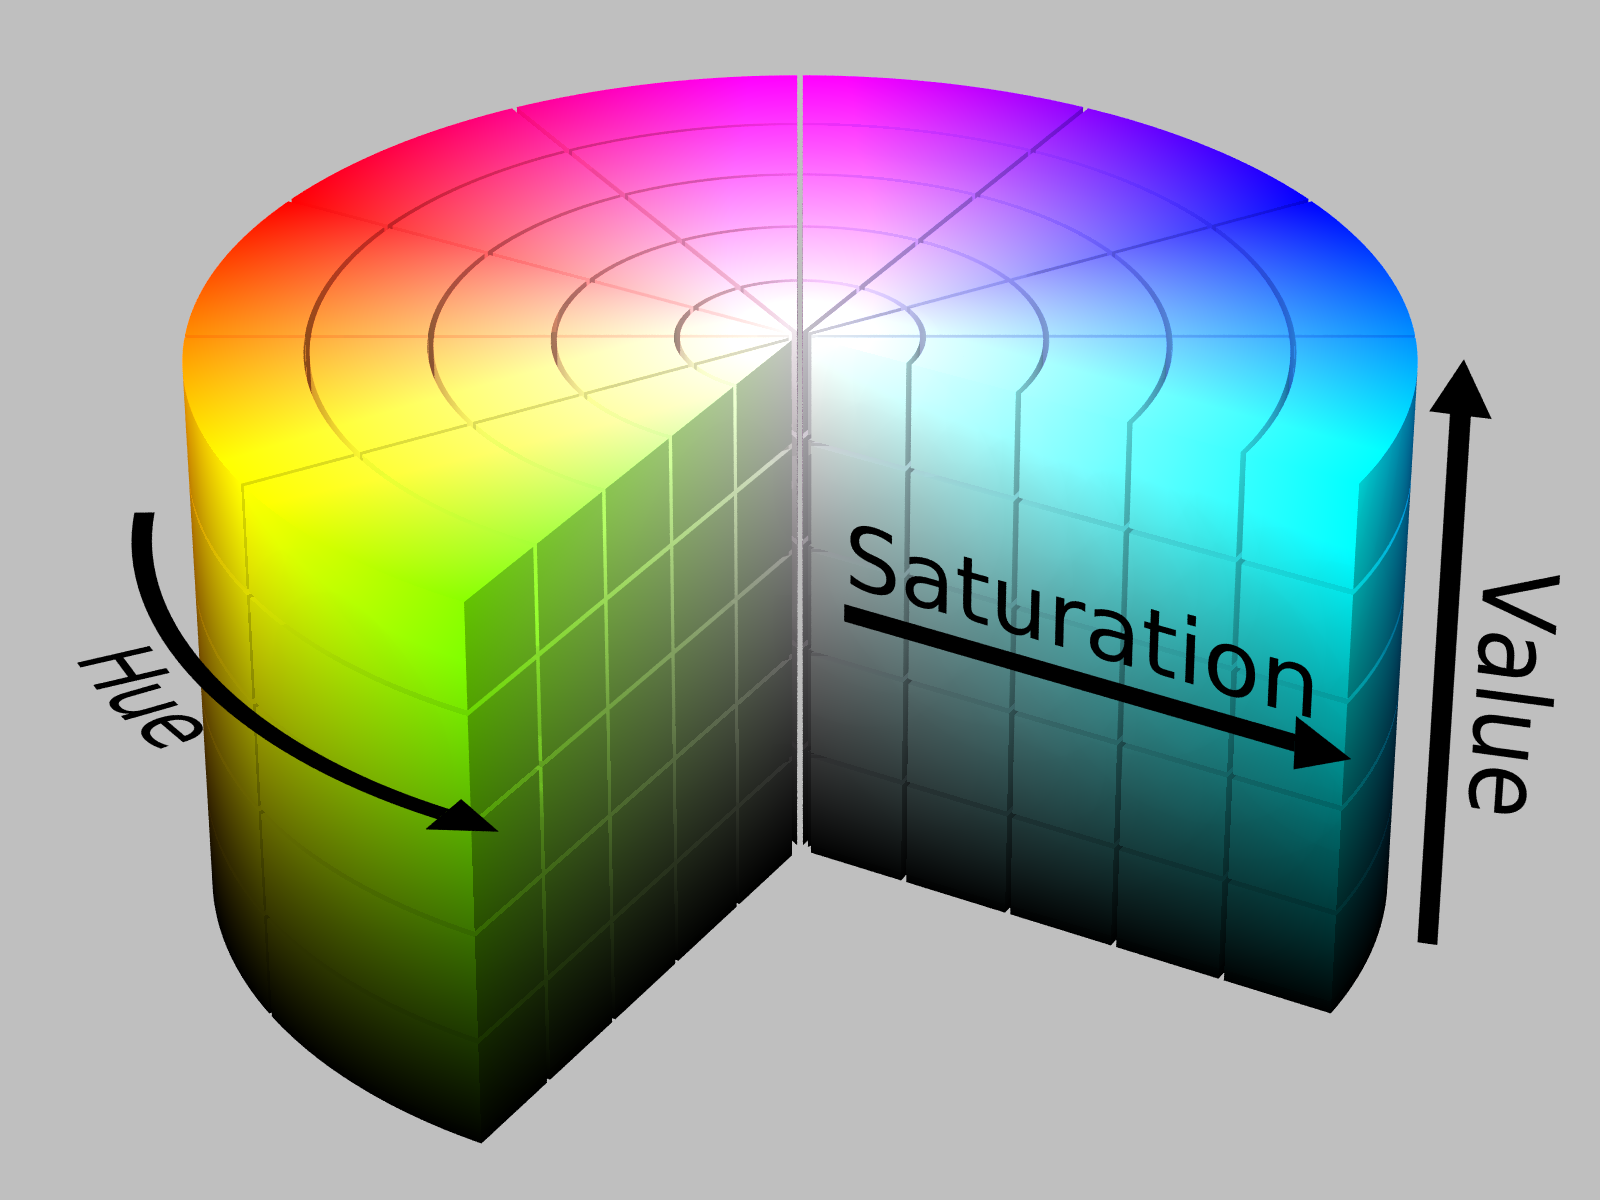
\includegraphics[scale=0.2]{../res/hsv.png}
\caption{HSV model boja \cite{bels5}}
\label{hsv}

\end{figure}

\subsection{Mapiranje pojedinih boja u frekvencije zvuka}

Sve pojave i događaji u prirodi uspješno se mogu opisati zakonima fizike, a usku vezu sa ovim zakonima dijele boje i zvukovi. Kao što je već rečeno, boje i zvukovi predstavljaju veoma bitne faktore koji djeluju na proces percepcije okoline od strane posmatrača. Iako svaki doživljaj okoline predstavlja subjektivnu pojavu, razvijene su mnoge metode korištene za analizu i manipulaciju ovim faktorima u cilju proučavanja procesa u kojem određeno živo biće sa čulima sluha i vidi percipira svoju okolinu. \\

U svrhu proučavanja ovih faktora i njihovog udjela u procesu percepcije, neophodno je bilo pronaći način na koji se oni predstavljaju. Poznato je da se i zvuk i boja mogu predstaviti \textbf{odgovarajućim frekvencijama} i upravo su proučavanjem ovih frekvencija izvedene mnoge analize i pronađena rješenja koja olakšavaju percepciju pojedincima sa oslabljenim čulom sluha ili vida. U ovom radu fokus je stavljen na način na koji se određena slika, koja se sastoji od određenog broja piksela, pretvara u zvučni sadržaj.  \\

Ovaj proces konverzije temelji se na predstavljanju boja od kojih je sastavljena posmatrana slika preko nekog od modela boja koji su opisani u prethodnom poglavlju. Nakon toga se vrši mapiranje odabranog modela u odgovarajuću zvučnu frekvenciju. U ovu svrhu, najčešće se koristi \textbf{HSV model boja} iz prostog razloga što predstavlja boje koje su najsličnije percepciji ljudskog oka. Kao što je već rečeno, HSV model boja se sastoji od tri kanala: \textit{Hue}, koji opisuje nijansu, \textit{Saturation}, koji opisuje zasićenost, te \textit{Value}, koji opisuje vrijednost. Na osnovu ovoga određen je način na koji se \textbf{svaki od ovih kanala mapira u odgovarajuću zvučnu karakteristiku}, što je prikazano na Slici \ref{HSVtoSound} \cite{n1}.

\begin{figure}[H]

\center
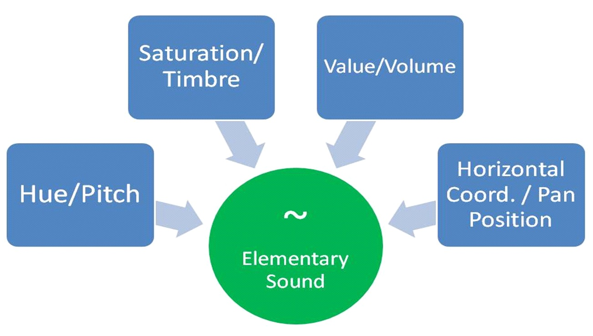
\includegraphics[scale=0.6]{../res/HSVtoSound.PNG}
\caption{Preslikavanje HSV modela boja u zvučne parametre \cite{n4}}
\label{HSVtoSound}

\end{figure}

Nijansa (\textit{Hue}) boje određuje količinu proizvedenih vibracija, odnosno \textbf{frekvenciju zvuka} (\textit{pitch}). Zasićenost (\textit{Saturation}) određuje \textbf{kvalitetu zvuka} (\textit{timbre}), dok je vrijednost (\textit{Value}) vezana za predstavljanje \textbf{jačine zvuka} (\textit{volume}). Četvrti parametar prikazan na Slici \ref{HSVtoSound} predstavlja horizontalne koordinate piksela koje se u ovom procesu konverzije preslikavaju u poziciju koja simulira položaj zvučnog izvora u horizontalnoj ravni. Na ovaj način se nastoji osigurati da se promjenom kanala boja u određenom smjeru, mijenja frekvencija zvuka, kvalitet kao i jačina zvuka, te time \textbf{preslikati percepciju} kojom ljudi povezuju zvuk sa određenim bojama \cite{n2}. \\

Veza između boje i zvuka oduvijek je bila zanimljiva tema istraživanja mnogim filozofima i naučnicima, a jedan od njih je i \textbf{Isaac Newton} \cite{n3}. U ovom radu će biti prikazan jedan način implementacije preslikavanja kanala boja u odgovarajuće zvučne parametre.

\subsection{Kreiranje zvučnog sadržaja na osnovu boja}

\subsubsection{Odabir audio formata}

Postoji veliki broj audio formata koji omogućavaju čuvanje zvučnih sadržaja nastalih prirodnim ili vještačkim putem, no većina takvih formata zahtijeva \textbf{uzorkovanje signala} te veliku preciznost kako bi izlazni \textit{file}-ovi bili dovoljno kvalitetni. S povećanjem broja uzoraka u jedinici vremena povećava se kvalitet zvučnog sadržaja, no u isto vrijeme, povećava se i \textbf{memorija potrebna za njihovo čuvanje}. \\

Prema Nyquistovom teoremu o uzorkovanju, frekvencija uzorkovanja signala mora biti barem dva puta veća od kritične frekvencije prisutne u izvornom signalu kako bi se signal mogao uspješno rekonstruisati. U slučaju zvuka, ljudski slušni sistem ima najvišu frekvenciju mehaničke rezonance u iznosu od \textbf{20 kHz}, te iz tog razloga frekvencija uzorkovanja treba biti \textbf{barem 40 kHz} kako ne bi došlo do pojave \textit{aliasinga} (pogrešne rekonstrukcije signala zbog nedovoljnog uzorkovanja) \cite{shupi}. Na Slici \ref{audioQualities} prikazan je trend porasta zauzeća memorije pri porastu kvaliteta prirodnih audio sadržaja, te je vidljivo da veći broj audio formata nema dovoljnu frekvenciju uzorkovanja za rekonstrukciju ulaznih zvučnih signala. \cite{dat}\\

\begin{figure}[H]

\center
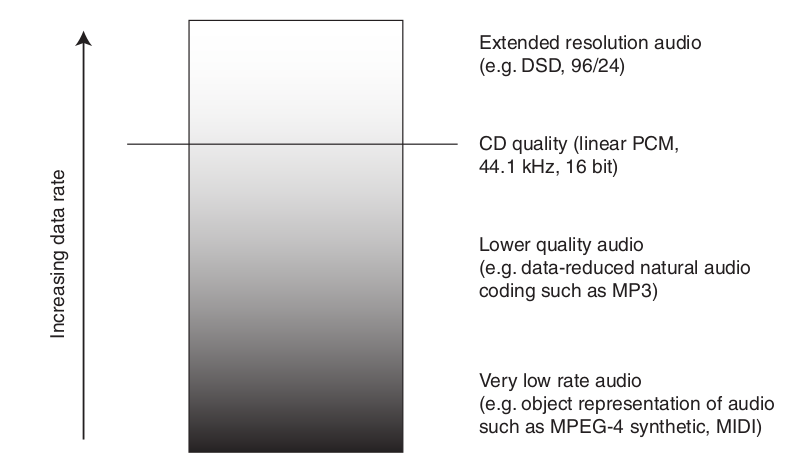
\includegraphics[scale=0.35]{../res/audioQualities.png}
\caption{Odnos količine podataka i frekvencije uzorkovanja audio signala \cite{dat}}
\label{audioQualities}

\end{figure}

U slučaju pretvaranja slika u zvučni sadržaj, nema razloga za korištenje audio formata koji imaju visoku frekvenciju uzorkovanja, odnosno koji su prilagođeni za uzorkovanje ulaznih signala (poput RIFF, PCM ili DSD formata), budući da je manja frekvencija uzorkovanja, tj. manja preciznost pri kvantizaciji, \textbf{sasvim dovoljna} kako bi vještački kreiran zvuk bio dovoljno kvalitetan. Jedan od formata koji je pogodan za ovakvu obradu je \textbf{MIDI format}, o kojem će biti više riječi u nastavku.

\subsubsection{\textit{Musical Instrument Digital Interface} format}

MIDI predstavlja protokol kreiran ranih 1980-ih godina kako bi se omogućilo \textbf{kontrolisanje muzičkih instrumenata} i svih njihovih aspekata (visina, jačina tona, pritisak na tipku, držanje tipke, ritam, sinkope i sl.), što nijedan prethodni format nije razmatrao. Glavna razlika između standardnih formata za digitalizaciju zvuka i MIDI formata je u tome što se u ovom formatu \textbf{ne čuvaju podaci o uzorcima zvučnog signala}, tako da se omogućava kreiranje \textit{file}-ova koji se ne sastoje od velikog broja uzoraka frekvencija zvuka u vremenu. \\

U ovom formatu, zvuk poprima jednu od \textbf{128 karakterističnih frekvencija} (odnosno, frekvencija predstavljenih 16-bitnim vrijednostima) odabranih za predstavljanje muzičkih nota (pri čemu je najniži ton C$_0$ kodiran heksadecimalnom vrijednošću \texttt{00 00}, te ima frekvenciju od 16.35 Hz, a najviši ton B$_9$ kodiran je heksadecimalnom vrijednošću \texttt{FF FF} i ima frekvenciju 15,804.26 Hz \cite{frequencies}). Na ovaj način postiže se da je veličina \textit{file}-ova koji koriste ovaj protokol \textbf{mala u odnosu na druge formate}, jer nema potrebe za čuvanjem velikog broja uzoraka po jedinici vremena, zbog čega je za posljedicu i veličina audio \textit{file}-ova koji koriste MIDI format manja u odnosu na druge audio formate. \cite{dat} \\

Posljedica mapiranja svih frekvencija zvuka u 128 karakterističnih frekvencija je \textbf{manji kvalitet zvuka}, no na ovaj način omogućava se kreiranje \textbf{potpuno vještačkog signala} (čemu je ovaj format primarno i namijenjen), što je veoma teško ili nemoguće izvršiti koristeći druge formate, budući da to nije njihova primarna namjena (već digitalizacija prirodnog zvučnog signala te što vjernije predstavljanje istog). \\

Još jedna važna razlika između MIDI formata i standardnih formata je u tome što je zvučni signal u standardnim formatima potpuno definisan, te je kao takav \textbf{na svim izlaznim uređajima uvijek isti}. MIDI format definiše veliki broj različitih aspekata važnih za izlazni signal i njegove pojedine dijelove, no sam ton (odnosno, karakteristična frekvencija) predstavlja samo \textbf{smjernicu} za konačni izlazni signal, što omogućava da se za isti ulazni \textit{file} dobiju različiti izlazni signali koristeći različite izlazne uređaje. Budući da su izlazni uređaji najčešće simulatori muzičkih instrumenata, na ovaj način postiže se jednostavna tranzicija između njih, te nije potrebno uvoditi dodatne specifikacije kako bi se omogućio ovaj efekat. Ovakvo nešto nemoguće je izvršiti koristeći standardne audio formate. \cite{dat} \\

U Tabeli \ref{TMIDI} prikazana je struktura kompletnog MIDI \textit{file}-a, o kojoj će biti riječi u nastavku.

\begin{table}[H]
\centering
\begin{tabular}{ | b b b b b | f f | e e |}
\hhline{---------}
\rowcolor{grey}
\multicolumn{5}{| c |}{\textit{MIDI Header}	}				& \multicolumn{2}{ c |}{\textit{Track Header}}		& \multicolumn{2}{ c |}{\textit{Track Data}}		\tabularnewline \hhline{-----|--|--}
4D 54 68 64	& 00 00 00 06 & 00 XX & D & E 				& 4D 54 72 6B 	& G								& [...] 	& 00 FF 2F 00							\tabularnewline \hhline{-----|--|--}
\end{tabular}
\caption{Struktura MIDI \textit{file}-a}
\label{TMIDI}
\end{table}

\textit{File}-ovi u MIDI formatu sastoje se od sljedećih dijelova \cite{midi}:

\begin{enumerate}

\item \textbf{\textit{MIDI Header}}, koji specificira format \textit{file}-a:

\begin{itemize}
\renewcommand\labelitemi{--}

\item \textbf{Sekcija A}: Označava da je format \textit{file}-a MIDI, te se sastoji od 4 \textit{byte}-a koji imaju heksadecimalnu vrijednost \texttt{4D 54 68 64};
\item \textbf{Sekcija B}: Specificira veličinu ostatka MIDI \textit{header}-a, odnosno broja \textit{byte}-a do početka informacija o samom signalu, te se sastoji od 4 \textit{byte}-a koji imaju heksadecimalnu vrijednost \texttt{00 00 00 06} (budući da ostali dijelovi \textit{header}-a imaju fiksnu dužinu);
\item \textbf{Sekcija C}: Označava tip MIDI formata. Postoje tri moguća tipa: \textit{tip 0} (osnovni tip), \textit{tip 1} (omogućava korištenje do 2$^16$ različitih \textit{channels} za definisanje različitih signala koji se pokreću u isto vrijeme) i \textit{tip 2} (koji predstavlja više MIDI \textit{file}-ova u jednom kako bi se definisali različiti šabloni zvuka). Ova sekcija sastoji se od 2 \textit{byte}-a (za najčešće korišteni tip 1, heksadecimalna vrijednost ove sekcije je \texttt{00 01});
\item \textbf{Sekcija D}: Označava broj \textit{channels} koji će se koristiti u \textit{file}-u, te se sastoji od 2 \textit{byte}-a;
\item \textbf{Sekcija E}: Označava brzinu signala, odnosno ritam zvuka, te se sastoji od 2 \textit{byte}-a.

\end{itemize}

U Tabeli \ref{MHeader} prikazana je struktura ovog dijela MIDI \textit{file}-ova.

\begin{table}[H]
\centering
\begin{tabular}{ | a a a a | b b b b | d d | e e | f f |}
\hhline{--------------}
\rowcolor{grey}
\multicolumn{4}{| c |} A 				& \multicolumn{4}{c |} B 				& \multicolumn{2}{c |} C 		& \multicolumn{2}{c |} D 		& \multicolumn{2}{c |} E 	\tabularnewline \hhline{----|----|--|--|--}
4D 	& 54	& 68	& 64			& 00	& 00	& 00	& 06		& 00	& XX 				& YY	& YY				& ZZ	& ZZ			\tabularnewline \hhline{----|----|--|--|--}
\end{tabular}
\caption{Struktura MIDI \textit{header}-a}
\label{MHeader}
\end{table}

\item \textbf{\textit{Track Header}}, koji daje osnovne informacije o samom zvučnom signalu:

\begin{itemize}
\renewcommand\labelitemi{--}

\item \textbf{Sekcija F}: Označava početak podataka o zvučnom signalu, te se sastoji od 4 \textit{byte}-a koji imaju heksadecimalnu vrijednost \texttt{4D 54 72 6B};
\item \textbf{Sekcija G}: Specificira broj \textit{byte}-a u ostatku \textit{file}-a, odnosno veličinu samog zvučnog signala. Budući da se ova sekcija sastoji od 4 \textit{byte}-a, najveća moguća veličina zvučnog signala je 2$^32$ \textit{byte}-a.

\end{itemize}

U Tabeli \ref{THeader} prikazana je struktura ovog dijela MIDI \textit{file}-ova.

\begin{table}[H]
\centering
\begin{tabular}{ | e e e e | b b b b |}
\hhline{--------}
\rowcolor{grey}
\multicolumn{4}{| c |} F 				& \multicolumn{4}{c |} G 				\tabularnewline \hhline{----|----}
4D 	& 54	& 72	& 6B			& XX	& XX	& XX	& XX		\tabularnewline \hhline{----|----}
\end{tabular}
\caption{Struktura \textit{track header}-a}
\label{THeader}
\end{table}

\item \textbf{\textit{Track Data}}, koji sadrži sam signal, odnosno njegove pojedine dijelove (muzičke tonove). Svaki ton sastoji se iz sljedećih dijelova:

\begin{itemize}
\renewcommand\labelitemi{--}

\item \textbf{\textit{Timestamp}}: Označava broj vremenskih jedinica koje trebaju proći prije početka sljedećeg tona, odnosno njegovo kašnjenje. Za čekanja do 127 otkucaja (\texttt{7F}) ova sekcija sastoji se od jednog \textit{byte}-a. \\

Za sva veća čekanja, dodaje se po jedan \textit{byte} vrijednosti \texttt{81} koja se zatim povećava po potrebi (naprimjer, čekanje od 128 otkucaja specificira se kao \texttt{81 7F}, pri čemu se ne uvodi novi \textit{byte} dok se ne dostigne vrijednost \texttt{FF 7F} i sl.). \\

Razlog za ovakvo kodiranje je što je potrebno biti moguće kodirati velika kašnjenja, a u isto vrijeme treba se moći identificirati mjesto na kojem informacija o kašnjenju završava, što ne bi bilo moguće u slučaju da svi \textit{byte}-i mogu poprimiti vrijednosti od \texttt{00} do \texttt{FF};
\item \textbf{\textit{Status}}: Gornja četiri bita ovog \textit{byte}-a označavaju događaj (\textit{event}), odnosno akciju koju je potrebno izvršiti prije početka sljedećeg tona (moguće vrijednosti prikazane su u tabeli \ref{status}), dok donja četiri bita označavaju \textit{channel} na koji se sljedeći ton i sve specificirane postavke odnose.
\item \textbf{\textit{Pitch}}: Predstavlja karakterističnu frekvenciju, odnosno sljedeći ton u zvučnom signalu, te se sastoji od jednog \textit{byte}-a (vrijednosti od \texttt{00} do \texttt{7F});
\item \textbf{\textit{Volume}}: Predstavlja jačinu tona, te se sastoji od jednog \textit{byte}-a (vrijednosti od \texttt{00} do \texttt{7F}).

\end{itemize}

U Tabeli \ref{TData} prikazana je struktura ovog dijela MIDI \textit{file}-ova.

\begin{table}[H]
\centering
\begin{tabular}{ | b b | e f | d | a |}
\hhline{------}
\rowcolor{grey}
\multicolumn{2}{| c |}{\textit{Timestamp}}			& \multicolumn{2}{ c |}{\textit{Status}}				& \textit{Pitch}		& \textit{Volume} 				\tabularnewline \hhline{--|--|-|-}
[...] 	& XX									& Y		& Z											& AA				& BB							\tabularnewline \hhline{--|--|-|-}
\end{tabular}
\caption{Struktura pojedinih tonova}
\label{TData}
\end{table}

\begin{table}[H]
\centering
\begin{tabular}{| P{2.5 cm} | c |}
\hhline{--}
\rowcolor{grey}
Statusni bit 		& Značenje											\tabularnewline \hhline{-|-}
8				& Ugasi ton											\tabularnewline \hhline{-|-}
9				& Upali ton											\tabularnewline \hhline{-|-}
A 				& Pritisak tipke instrumenta (\textit{AfterTouch})			\tabularnewline \hhline{-|-}
B 				& Kontroler (simulacija fizičkih osobina uređaja) \cite{dat}	\tabularnewline \hhline{-|-}
C 				& Promjena programa (simulacija efekata) \cite{dat}		\tabularnewline \hhline{-|-}
D 				& Jačina pritiska na tipku								\tabularnewline \hhline{-|-}
E 				& Visina tona											\tabularnewline \hhline{-|-}
\end{tabular}
\caption{Moguće vrijednosti statusnih bita}
\label{status}
\end{table}

Važno je napomenuti da se nakon posljednjeg tona mora definisati kraj zvučnog sadržaja ubacivanjem vrijednosti \texttt{00 FF 2F 00}. Ovo je jedna od formi \textit{meta events}, odnosno lažnih događaja koji se kodiraju na isti način kao i stvarni događaji koji proizvode tonove, no kao posljedicu nemaju novi ton, već neku drugu akciju. Svi lažni događaji sastoje se iz četiri dijela:

\begin{itemize}
\renewcommand\labelitemi{--}

\item Prvi \textit{byte} označava da je u pitanju \textit{meta event} i uvijek ima heksadecimalnu vrijednost \texttt{FF};
\item Drugi \textit{byte} specificira vrstu \textit{meta event}-a (informacije o samom \textit{file}-u (broj snimka, autor, godina, ime kompozicije i sl.), tempo, MIDI port, itd.) \cite{dat};
\item Treći dio specificira broj \textit{byte}-a od kojih se sami podaci sastoje;
\item Četvrti dio sadrži same podatke.

\end{itemize}

U Tabeli \ref{TMetadata} prikazana je struktura ovog dijela MIDI \textit{file}-ova.

\begin{table}[H]
\centering
\begin{tabular}{ | f | d | a | b |}
\hhline{----}
\rowcolor{grey}
1			& 2				& 3			& 4 				\tabularnewline \hhline{-|-|-|-}
FF 			& XX			& YY		& [...]			\tabularnewline \hhline{-|-|-|-}
\end{tabular}
\caption{Struktura \textit{meta event}-a}
\label{TMetadata}
\end{table}

\end{enumerate}

\newpage

\section{Implementacija rješenja problema}

\subsection{Manipulacija slikom}

Za svrhu pretvaranja boje u odgovarajući ton, kreirane su dvije funkcije: \texttt{toNormalizedHue}, te \texttt{imageToSound}, koje obje kao parametar primaju putanju do željene slike. Funkcija \texttt{toNorma- lizedHue} prikazana u Listingu \ref{image1} pretvara odabranu sliku u niz \textbf{pogodan za biranje tona boje}, koji je opisan u narednim poglavljima. Kako je potrebno vrijednosti piksela pretvoriti u cjelobrojne vrijednosti u intervalu [0,128), korišten je \textbf{HSV model}, tačnije, kanal nijanse (\textit{hue}), koji je potom skaliran. Bitno je napomenuti da RGB model \textbf{nije korišten} zbog kompleksnosti mapiranja boja u dati interval, te da se sa \textit{grayscale} slikama gubi smisao pretvaranja boje u zvuk. \\
~\\
Kako će veće slike rezultirati većim audio zapisom, korištena je ideja dobivena iz \textbf{DCT algoritma}: \underline{blokovi slike su kodirani u jedinstvenu notu}, tako što se uzela prosječna vrijednost piksela. Ovisno od veličine slike, vrijednosti varijable \texttt{factor}, koja predstavlja veličinu bloka, variraju \textbf{od 8 do 64}. Nakon računanja prosječne vrijednosti blokova, podaci su kopirani u odgovarajući tip, te se šalju na dalje procesiranje.

\begin{lstlisting}[language={[Sharp]C}, caption={Funkcija \texttt{toNormalizedHue} za pretvaranje boja u tonove}, label={image1}]
//helper function to turn image to normalized hue
static int[,] toNormalizedHue(string path) //path to image
{
		Bitmap bitmap = new Bitmap(path); //load image
		int width = bitmap.Width;
		int height = bitmap.Height;
		int[,] note = new int[height, width]; //all of the values [0,128) will  be stored here
		for (int i = 0; i < height; i++) {
			for (int j = 0; j < width; j++) {
				Color pixel = bitmap.GetPixel(j, i);
                   		float hue = pixel.GetHue(); //get Hue of pixel
                   		hue = hue * 127F / 360F; //normalise to [0,128)
                   		note[i, j] = (int)(Math.Floor(hue)); //round to int
			}
		}
		//since large images will produce longer audio files, the factor variable is introduced
		//similar to DCT, we will use blocks of the image to shorten the audio file
		//bigger images will have a bigger factor
		List<List<int>> notes = new List<List<int>>();
		int factor = 8;
		if (width > 2500 || height > 2500) {
			factor = 64;
		}
		else if (width > 1500 || height > 1500) {
			factor = 32;
		}
		else if (width > 1000 || height > 1000) {
			factor = 16;
		}
		//calculating average normalized hue value for blocks size (factor x factor)
		for (int i = 0; i < height; i += factor) {
			List<int> temp = new List<int>();
			for (int j = 0; j < width; j += factor) {
				double sum = 0;
     //total is kept track of since it is possible that a whole block would not fit in (instead of padding the image)
                    	int total = 0;
                    	for (int k = i; k < i + factor && k < height; k++) {
					for (int l = j; l < j + factor && l < width; l++) {
						sum += note[k, l];
						total++;
					}
                    	}
                    	temp.Add((int)(Math.Floor(sum / total)) + 1);
                    	sum = 0;
                    	total = 0;
			}	
			notes.Add(temp);
		}
		//copying to the needed return type
		int[,] returnNote = new int[notes.Count, notes[0].Count];
		for (int i = 0; i < returnNote.GetLength(0); i++) {
			for (int j = 0; j < returnNote.GetLength(1); j++) {
				returnNote[i, j] = notes[i][j];
			}
		}
		return returnNote;
}
\end{lstlisting}
~\\
Funkcija \texttt{imageToSound} prikazana u Listingu \ref{image2} pretvara odabranu sliku u zvučni zapis uz pomoć klase \texttt{MIDIFIle} opisane u nastavku. Nakon što se pozove \texttt{toNormalizedHue}, dobiveni dvodimenzionalni niz \textbf{dodaje za svaki piksel notu} metodom \texttt{addNote}, nakon čega se kreira audio zapis uz pomoć metode \texttt{createMIDIFile} (u nastavku su objašnjene pomenute metode).

\begin{lstlisting}[language={[Sharp]C}, caption={Funkcija \texttt{imageToSound} za kreiranje audio \textit{file}-a}, label={image2}]
static void imageToSound(string path) //path to image
{
            MIDIFile m = new MIDIFile();
            int[,] note = toNormalizedHue(path);
            m.setVolume(127);
            for (int i = 0; i < note.GetLength(0); i++) {
                for (int j = 0; j < note.GetLength(1); j++) {
                    m.addNote(note[i, j]); //create MIDI file of notes acquired from the hue channel of the image
                }
            }
            m.createMIDIFile("test"); //create MIDI file
}
\end{lstlisting}

\newpage

\subsection{Manipulacija zvukom}

Treća faza konverzije slika u boji u zvuk je \textbf{kreiranje MIDI \textit{file}-a} s tonovima koji predstavljaju odgovarajuće boje od kojih se slika sastoji. Kako bi se to omogućilo, kreirana je klasa \texttt{MIDIFile}, čiji atributi predstavljaju pojedine dijelove MIDI \textit{file}-a koji se sukcesivno kreira, odnosno koji ima predefinisane dijelove (\textit{header} dijelove), a dio koji se odnosi na same podatke (tj. tonove) inicijalno je prazan. Atributi klase \texttt{MIDIFile} prikazani su u Listingu \ref{MIDIclass}.

\begin{lstlisting}[language={[Sharp]C}, caption={Klasa MIDIFile i njeni atributi}, label={MIDIclass}]
public class MIDIFile
    {
        #region MIDIHeader
        string format = "4D546864"; // specifies that the file format is MIDI (MThd)
        string headerSize = "00000006"; // specifies the number of bytes of
                    // the following three parts of the MIDI header (SMF)
        string type = "0001"; // specifies the type of MIDI (0, 1 or 2)
        string tracks = "0001"; // specifies the number of tracks (0 - 65.536)
        string speed = "0080"; // specifies the speed of music
        #endregion
        #region TrackHeader
        string start = "4D54726B"; // specifies the track start (MTrk)
        string noOfBytes = ""; // specifies the number of bytes in the track
        #endregion
        #region Track
        string data = ""; // specifies the musical notes in the track
        string rhythm = "8100"; // specifies the speed of each note
        string volume = "60"; // specifies the volume of each note
        string end = "00FF2F00"; // specifies the track end
        #endregion
    }
\end{lstlisting}
~\\
Klasa \texttt{MIDIFile} omogućava \textbf{dodavanje novog tona} na vrlo jednostavan način. Kao parametar se prima cjelobrojna vrijednost između 0 i 127 (koja predstavlja karakterističnu frekvenciju tona), te se zatim provjerava da li je u pitanju prvi ton ili ne. Ukoliko je u pitanju prvi ton, potrebno je poslati signal da se pritišće prva tipka, dok je u svakom drugom slučaju dovoljno dodati samo broj otkucaja koji se čekaju do početka sljedećeg tona. Zatim se dodaje vrijednost koja označava karakterističnu frekvenciju (uz dodatnu provjeru da li karakteristična vrijednost ima dva \textit{byte}-a, te ukoliko nema, drugi \textit{byte} se manuelno dodaje), te trenutno postavljena vrijednost jačine zvuka. Ova funkcionalnost implementirana je u funkciji \texttt{addNote}, čija je struktura prikazana u Listingu \ref{MIDInote}.

\begin{lstlisting}[language={[Sharp]C}, caption={Metoda za dodavanje tonova u MIDI \textit{file}}, label={MIDInote}]
// adds a new note (range from 0 to 127) to the track
        public void addNote(int note)
        {
            if (data.Length == 0) data += "800090"; // the first note needs
                            // to send the signal to turn the notes on
            else data += rhythm;
            if (note < 16) data += "0";
            data += note.ToString("X") + volume;
        }
\end{lstlisting}
~\\
Nakon dodavanja svih željenih tonova, potrebno je kreirati \textit{.mid file} koji se sastoji od svih prethodno navedenih dijelova. Nakon dodavanja posljednjeg, ''tihog'' tona koji signalizira otpuštanje pritiska na tipku, svi dijelovi (\textit{headers} i \textit{data}) sastavljaju se u \textbf{jedinstvenu varijablu} koja se sastoji od heksadecimalnih vrijednosti prikazanih u obliku karaktera. Ti karakteri zatim se pretvaraju u binarne vrijednosti (2 po 2 karaktera, kako bi se dobila 16-bitna vrijednost) koje se redom upisuju u \textbf{binarni \textit{file} s ekstenzijom \textit{.mid}}. Ova funkcionalnost implementirana je u funkciji \texttt{createMIDIFile}, čija je struktura prikazana u Listingu \ref{MIDIfile}.

\begin{lstlisting}[language={[Sharp]C}, caption={Spajanje svih dijelova MIDI \textit{file}-a i kreiranje \textit{.mid file}-a}, label={MIDIfile}]
        // puts all file parts together and writes to .mid file
        public void createMIDIFile(string path)
        {
            data += rhythm + "B07B00"; // the final note just turns off the music
            noOfBytes = ((data.Length + end.Length) / 2).ToString("X");
            			// previously skipped part of TrackHeader
            while (noOfBytes.Length < 8) noOfBytes = "0" + noOfBytes;
            			// the noOfBytes part needs to have 8 bytes
            string file = format + headerSize + type + tracks + speed +
                          start + noOfBytes + data + end; // putting all parts together
            // writing to .mid file - hexadecimal code is converted to binary and then written to file
            var stream = new FileStream(path + ".mid", FileMode.Create, FileAccess.ReadWrite);
            var twoCharacters = new StringBuilder(); // two bytes are used for every conversion (16 bits - two hex numbers)
            var singleByte = new byte[1]; // two binary bytes to which the hex numbers will be converted
            foreach (var character in file)
            {
                twoCharacters.Append(character); // adding one hex character to the 16-bit variable
                if (twoCharacters.Length == 2) // added two characters - reached 16 bits
                {
                    singleByte[0] = (byte)Convert.ToByte(twoCharacters.ToString(), 16); // conversion from hex to bin
                    stream.Write(singleByte, 0, 1); // writing bin to file
                    twoCharacters.Clear(); // starting over again with new characters
                }
            }
            stream.Close();
        }
\end{lstlisting}

\subsection{Aplikacija za pretvaranje slika u boji u zvučni sadržaj}

Nakon što su analizirani, opisani i implementirani pojedinačni dijelovi manipulacije nad slikom i zvukom, u ovom dijelu će biti opisano povezivanje svih komponenti u \textbf{jednu cjelinu} koju čini \textit{desktop} aplikacija. Aplikacija je implementirana upotrebom \textit{Windows Forms} projekta u okviru \textit{Visual Studio} razvojnog okruženja. \\
Implementirano rješenje sastoji se od \textbf{dva projekta}, kako je prikazano u \textit{Visual Studio Solution Explorer}-u na Slici \ref{solution}.

\begin{figure}[H]

\center
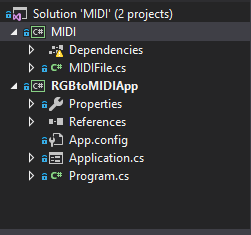
\includegraphics[scale=0.7]{../res/solution.png}
\caption{Projekti od kojih se aplikacija sastoji}
\label{solution}

\end{figure}

Prvi projekat pod nazivom \textbf{\texttt{MIDI}} predstavlja biblioteku klasa (\textit{Class Library}) i sastoji se od metoda pomoću kojih se dodaju note te kreira odgovarajući MIDI \textit{file}. Drugi projekat je \textbf{\textit{Windows Forms} projekat} u kojem je dizajniran izgled aplikacije i implementirana logika upravljanja korisničkim kontrolama. Na Slici \ref{app} prikazan je izgled aplikacije.

\begin{figure}[H]

\center
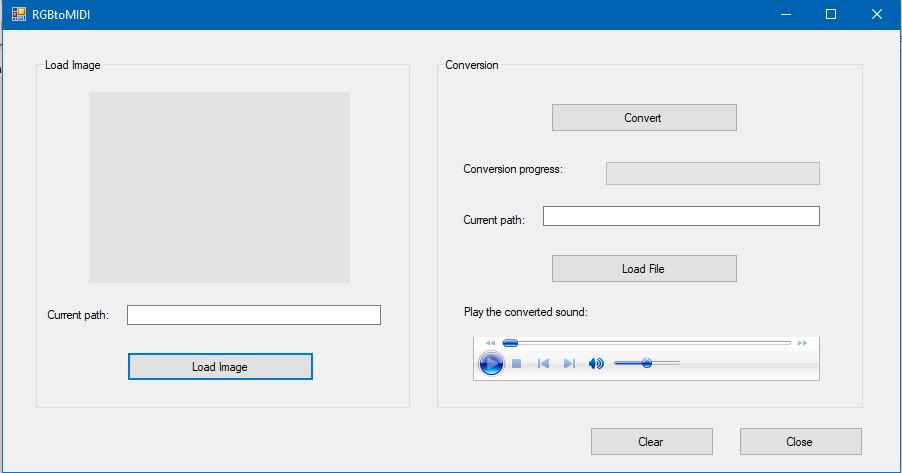
\includegraphics[scale=0.65]{../res/app.png}
\caption{Izgled aplikacije}
\label{app}

\end{figure}

Nakon pokretanja aplikacije, korisniku se otvara forma sa odgovarajućim korisničkim kontrolama. Klikom na dugme \textit{Load Image}, korisniku je omogućen \textbf{odabir željene slike za konverziju}. Nakon učitavanja slike, klikom na dugme \textit{Convert} vrši se \textbf{konverzija odabrane slike u MIDI \textit{file}}, pri čemu je putanja do kreirane datoteke prikazana u tekst polju na aplikaciji. \\

Ako je konverzija uspješno završena, korisniku se omogućava \textbf{učitavanje kreiranog \textit{file}-a}. Kreirani MIDI \textit{file} se može reproducirati u samoj aplikaciji pomoću \textit{Windows Media Player} korisničke kontrole. Dok se vrši konverzija, moguće je pratiti progres napretka pomoću \textit{Progress Bar} korisničke kontrole. Progres pri konverziji nakon odabira slike, kao i putanja \textit{file}-a u koji će se konverzija snimiti prikazani su na Slici \ref{workingApp}.

\begin{figure}[H]

\center
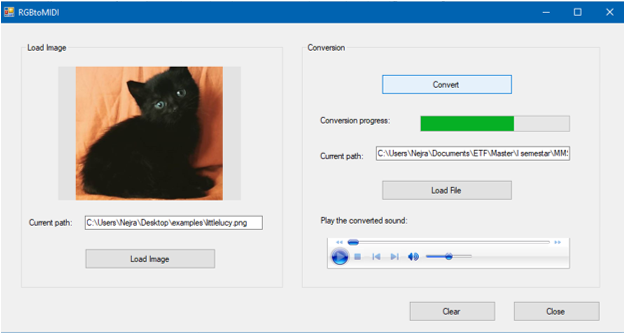
\includegraphics[scale=0.95]{../res/workingApp.PNG}
\caption{Izgled aplikacije tokom izvršavanja procesa konverzije}
\label{workingApp}

\end{figure}

Pored osnovne implementacije upravljanja događajima na korisničkim kontrolama, za ovaj rad su od najvećeg značaja dijelovi implementacije aplikacije vezani za \textbf{objedinjavanje implementiranih komponenti u jednu cjelinu}. Ti događaji se dešavaju klikom na dugme za konverziju i reproduciranjem \textit{file}-a. \\

U Listingu \ref{APPconvert} prikazano je upravljanje klikom na dugme \textit{Convert}. Dakle, postavljaju se odgovarajuće vrijednosti za \textit{Progress Bar} kontrolu, te se poziva \textbf{odgovarajuća nit} koja obavlja konverziju odabrane slike u MIDI \textit{file}.

\begin{lstlisting}[language={[Sharp]C}, caption={Pokretanje konverzije slike u audio \textit{file}}, label={APPconvert}]
private void buttonConvert_Click(object sender, EventArgs e)
        {
            progressBar1.Maximum = 100;
            progressBar1.Step = 1;
            progressBar1.Value = 0;
            backgroundWorker1.RunWorkerAsync();
        }
\end{lstlisting}
~\\

U Listingu \ref{APPbackground} prikazane su ostale operacije vezane za pokretanje niti za konverziju slike, pozivanje metode za pomenutu konverziju koja je opisana u jednom od prethodnih poglavlja, kao i ažuriranje \textit{Progress Bar}-a i korisničkih kontrola kada se konverzija završi.

\begin{lstlisting}[language={[Sharp]C}, caption={Vršenje konverzije u zasebnoj niti}, label={APPbackground}]
//turn hue to sound
        private void backgroundWorker1_DoWork_1(object sender, DoWorkEventArgs e)
        {
            var backgroundWorker = sender as BackgroundWorker;
            MIDIFile m = new MIDIFile();
            int[,] note = toNormalizedHue(imagePath);
            m.setVolume(127);
            int noOfSteps = note.GetLength(0) * note.GetLength(1);
            int reportProgressStep = noOfSteps / 100 + 1;
            int step = 0;
            for (int i = 0; i < note.GetLength(0); i++)  {
                for (int j = 0; j < note.GetLength(1); j++) {
                    m.addNote(note[i, j]); //create MIDI file of notes acquired from the hue channel of the image
                    step++;
                    if (step \% reportProgressStep == 0) backgroundWorker.ReportProgress(step / reportProgressStep);
                }
            }
            m.createMIDIFile("test"); //create MIDI file
            backgroundWorker.ReportProgress(100);
            musicFilePath = Directory.GetCurrentDirectory() + "\\test.mid";
        }

        private void backgroundWorker1_ProgressChanged_1(object sender, ProgressChangedEventArgs e)
        {
            progressBar1.Value = e.ProgressPercentage;
        }

        private void backgroundWorker1_RunWorkerCompleted(object sender, RunWorkerCompletedEventArgs e)
        {
            textBox1.Text = musicFilePath;
            string x = textBox1.Text;
        }
    }
\end{lstlisting}
~\\

Nakon što se \textit{file} uspješno kreira, implementacija koja omogućava njegovo pokretanje prikazana je u Listingu \ref{APPwmp}.

\begin{lstlisting}[language={[Sharp]C}, caption={Pokretanje reprodukcije MIDI \textit{file}-a}, label={APPwmp}]
private void axWindowsMediaPlayerPlay_Enter(object sender, EventArgs e)
        {
            axWindowsMediaPlayerPlay.URL = musicFilePath;
        }
\end{lstlisting}
~\\

Dakle, implementirana \textit{desktop} aplikacija spaja dijelove implementacije u jednu cjelinu i na jednostavan način omogućava pokretanje tih dijelova i prikaz rezultata njihovog rada. Cijela implementacija dostupna je na linku: \href{https://github.com/ehlymana/RGBtoMIDI}{https://github.com/ehlymana/RGBtoMIDI}.

\newpage

\section{Zaključak}

Razvoj tehnologije omogućio je jednostavnu i brzu manipulaciju multimedijalnim sadržajima. Postoji veliki broj različitih formata slika te gotovih programskih rješenja i biblioteka koje omogućavaju njihovu analizu, izmjenu ili ekstrakciju onih dijelova koji su važni za određenu primjenu. S druge strane, iako je obrada zvukom manje popularna, postoji veliki broj audio formata koji omogućavaju tretiranje zvuka na različite načine, kompresiju ili kreiranje potpuno vještačkih zvučnih signala, što također može biti korisno i od velike pomoći za različite primjene. Najvažnije je omogućavanje izvršavanja svih ovih obrada \textbf{u realnom vremenu}, što otvara vrata velikom broju mogućnosti. \\

Jedna od takvih mogućnosti je učitavanje slike, njeno razlaganje na \textit{color channels} te njihovo pretvaranje u audio \textit{file} koji je moguće reproducirati gotovo odmah. Na ovaj način omogućava se da boje, koje neki ljudi nisu u stanju vidjeti, budu pretvorene u karakterističnu frekvenciju koja, na isti način kao što oko prepoznaje karakteristične boje, bude prepoznata od strane slušnog sistema. Na ovaj način moguće je ukloniti prepreku koju predstavlja \textbf{nemogućnost viđenja boja}, odnosno omogućiti ljudima koji nisu u stanju da razlikuju boje (daltonizam) ili koji vide samo nijanse sive boje (ahromatopsija) da \textbf{''čuju'' boje}, odnosno da razlikuju boje na osnovu različite frekvencije zvuka koja se proizvodi na osnovu mapiranja boja u muzičke tonove. \\

Naravno, ovakav sistem nije savršen, jer postoji na milione različitih nijansi koje je ljudsko oko u stanju razlikovati, dok postoji samo 128 različitih muzičkih tonova, čime se većina nijansi zapravo \textbf{aproksimira} u jednu od karakterističnih frekvencija. Ovo je posljedica činjenice da vidni i čulni sistemi ne funkcionišu na isti način: u bazelarnoj membrani dolazi do pojave \textbf{frekvencijskog maskiranja}, pri čemu se bliske frekvencije detektuju kao jedna, što predstavlja jednu vrstu aproksimacije \cite{shupi}. Iz ovog razloga i postoji samo 128 različitih muzičkih tonova, zbog čega se nameće zaključak da je vršenje aproksimacija \textbf{neizbježno} pri mapiranju boja u frekvencije zvuka. \\

Iako je potpuno preslikavanje skupa boja u skup zvukova nemoguće, preslikavanje 128 boja je ipak dovoljno detaljan postupak kako bi se stvorio osjećaj razlikovanja boja. Na ovaj način omogućava se pojava \textbf{sinestezije}, odnosno nakon određenog vremena korištenja sistema za pretvaranje slika u boji u zvukove, ljudski čulni sistem koji nije u mogućnosti razlikovati boje početi će vršiti automatsku identifikaciju boja koje ne vidi na osnovu zvuka koji čuje. Omogućavanje viđenja boja i u slučaju kada je čulni organ oštećen ili defektan, bez obzira s kolikom aproksimacijom, veliki je uspjeh, jer može predstavljati veliku pomoć ljudima koji nisu u stanju razlikovati ili vidjeti boje, a za realizaciju ovakvog sistema nisu potrebne velike sume novca niti komplikovani postupci.

\newpage

\bibliographystyle{IEEEtran}
\bibliography{bibliography}

\end{document}